\documentclass[accentcolor=tud1b,colorbacktitle,landscape,german,presentation]{tudbeamer}

%Includes
\usepackage{float}
\usepackage{listings}
\usepackage{color}
\usepackage{graphicx}
\usepackage{epstopdf}
\usepackage{wrapfig}
%Deutsche Silbentrennung
\usepackage[ngerman]{babel}
%Deutsche Umlaute
\usepackage[utf8]{inputenc}
\usepackage{adjustbox}
\usepackage{hyperref}

\DeclareGraphicsExtensions{.pdf,.png,.jpg}
\graphicspath{ {./img/} }

\title[]{Steuerungsprogramm für den \\Forschungsflugsimulator}
\subtitle{{\scriptsize Frederik Bark, Heiko Carrasco, Jonas Meurer, Tim Weißmantel, Leonardo Zaninelli}}
\institute{BP WS 2017/18 | Institut für Flugsysteme und Regelungstechnik}
\date{\today}

\newcommand{\ftitle}{

	\frametitle{\insertsectionhead \\ {\small \insertsubsectionhead}}
}

\begin{document}

%Deckblatt
\begin{titleframe}
	\vspace{-2.4mm}
	\begin{figure}
		\centering
		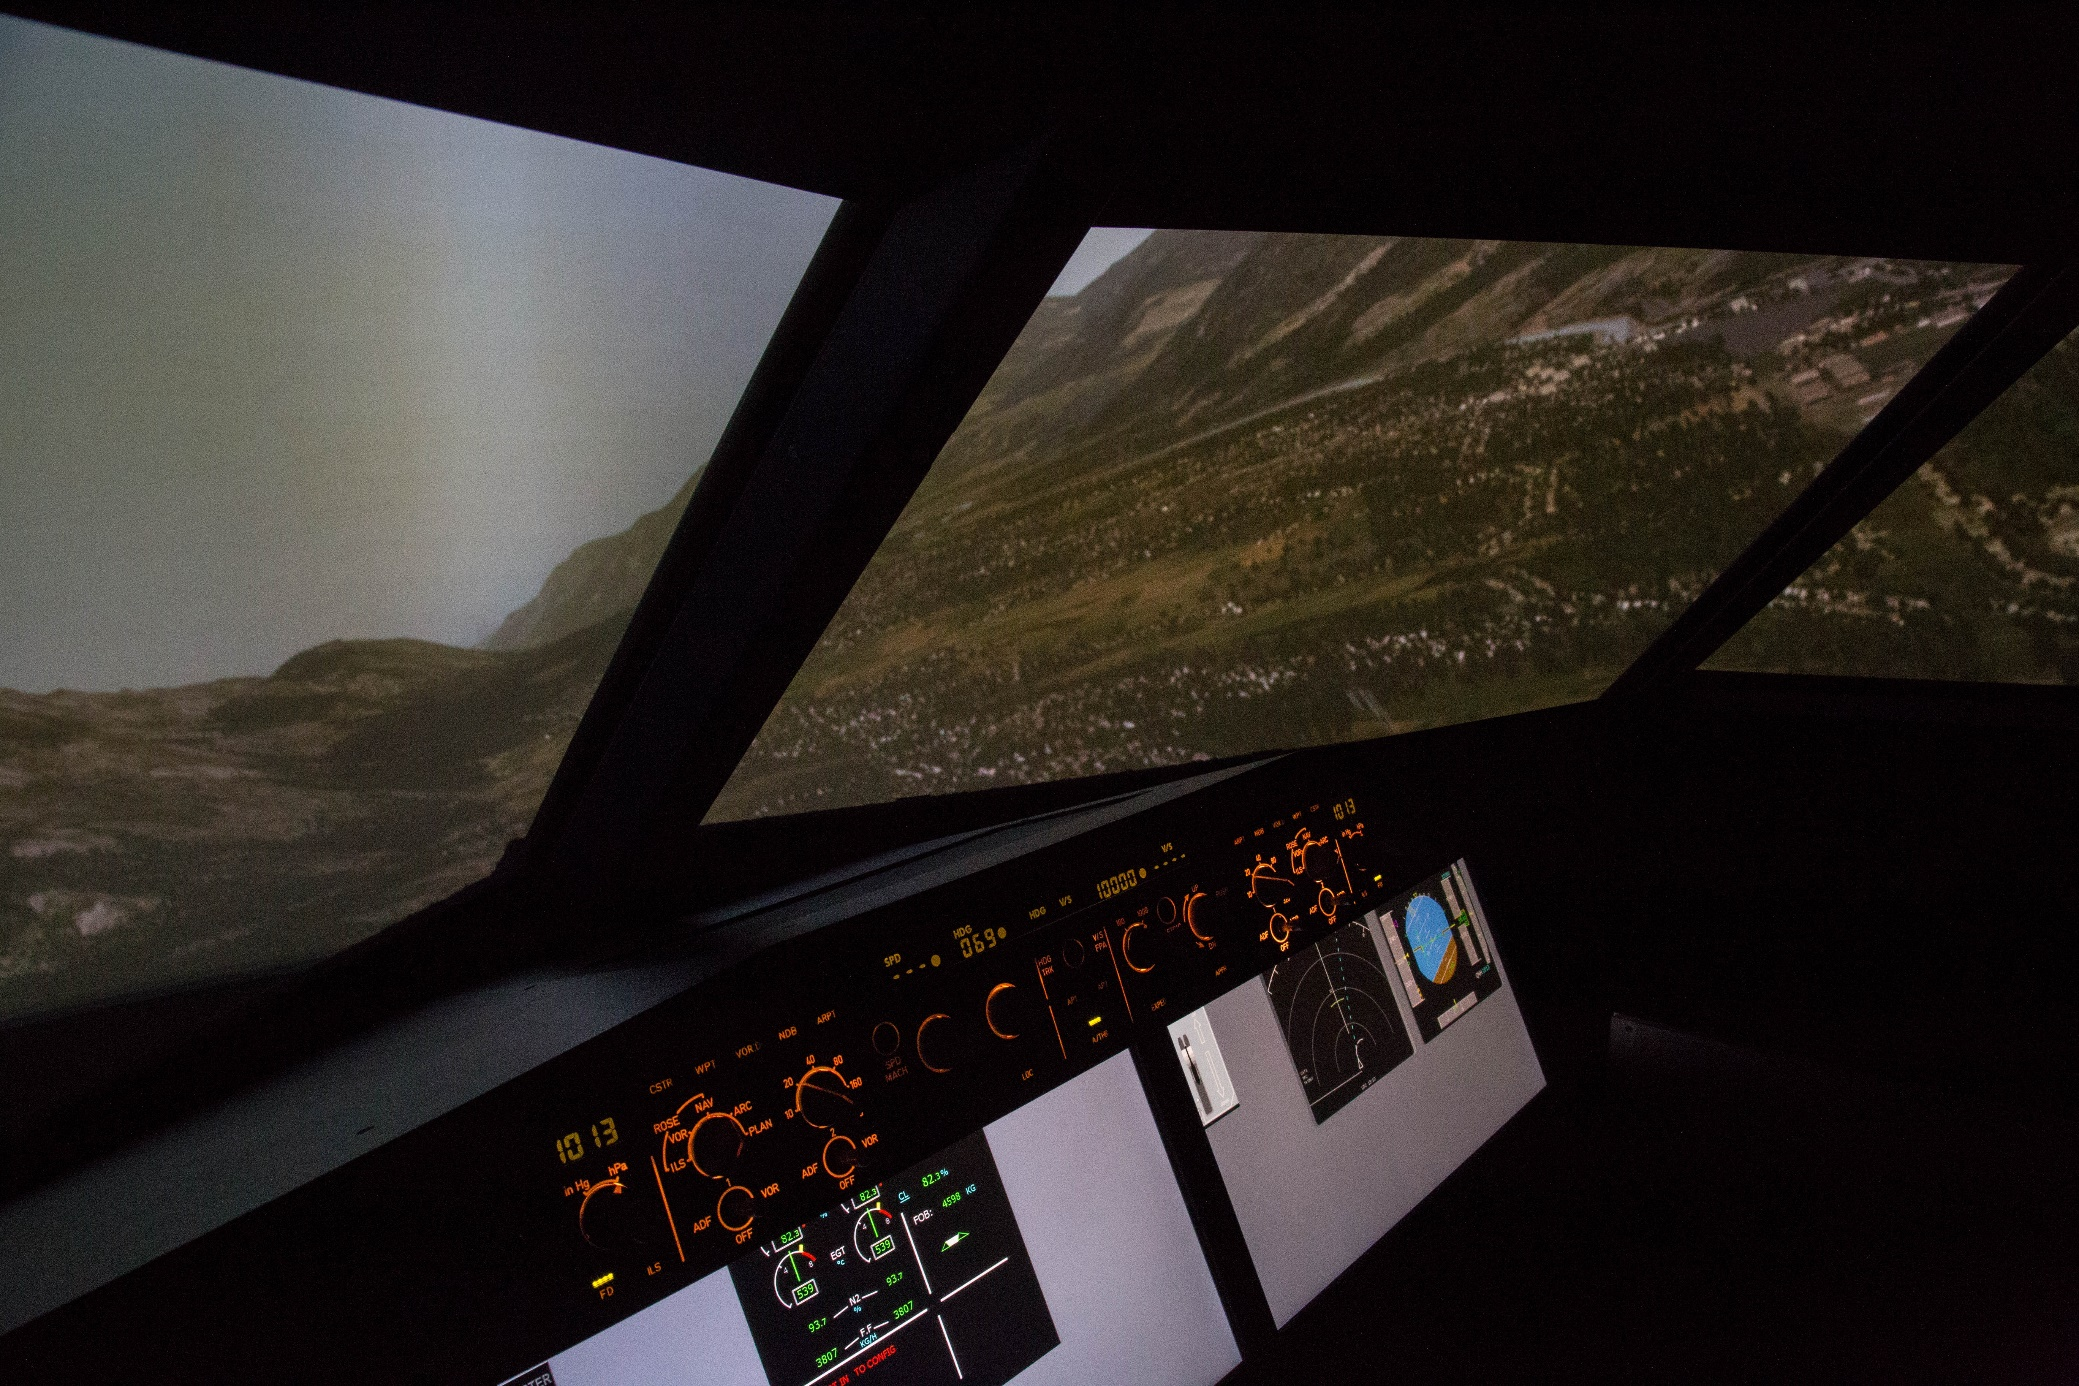
\includegraphics[scale=0.36]{simulator}
	\end{figure}
\end{titleframe}

\section{Software}
\subsection{Aufbau}

\begin{frame}
	\ftitle
	\begin{itemize}
		\item Client-Master System mit zentralem Server
	\end{itemize}
	\pause
	\begin{figure}
		\centering
		\only<2>{
\includegraphics[scale=0.42]{1}}
		\only<3>{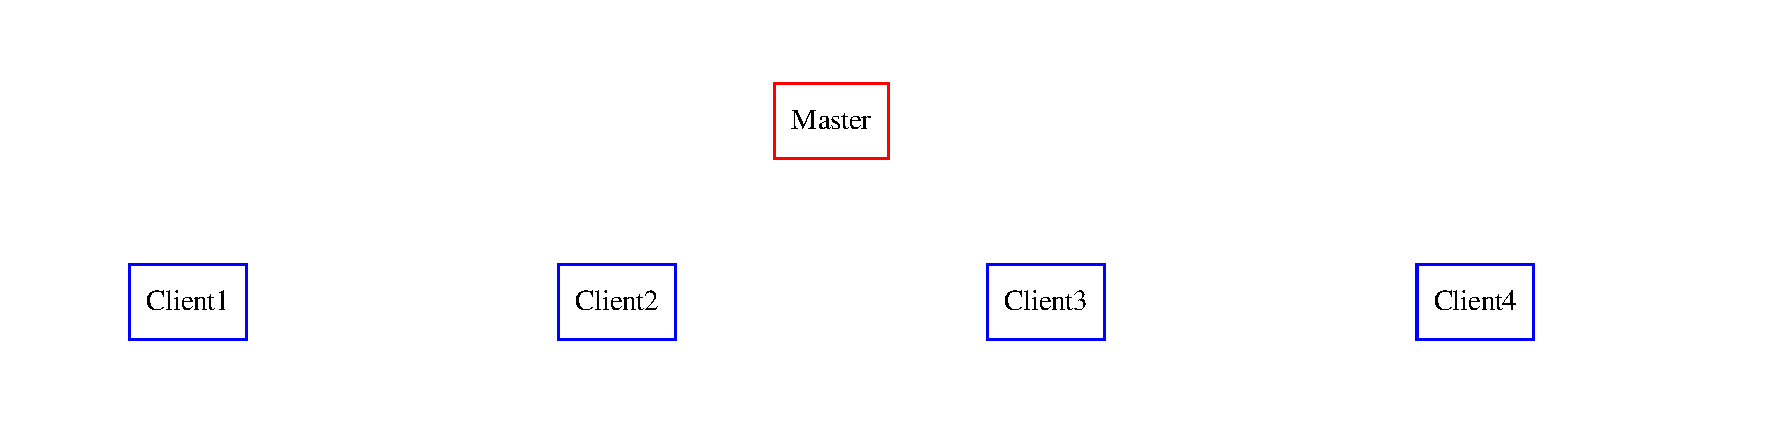
\includegraphics[scale=0.42]{2}}
		\only<4>{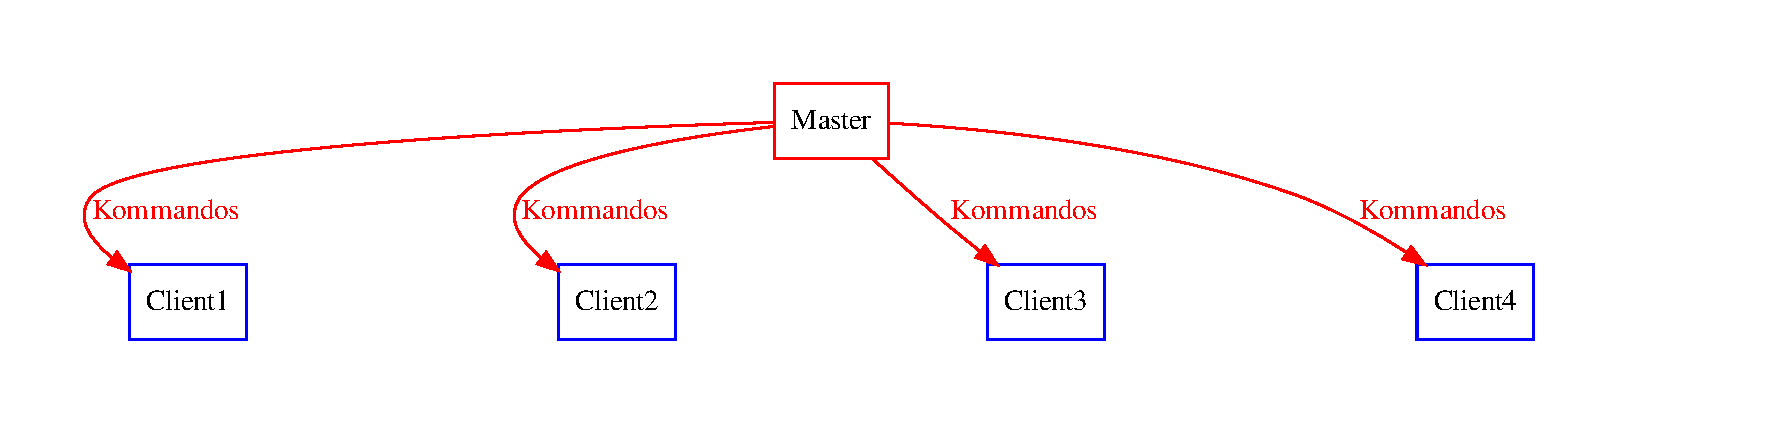
\includegraphics[scale=0.42]{3}}
		\only<5>{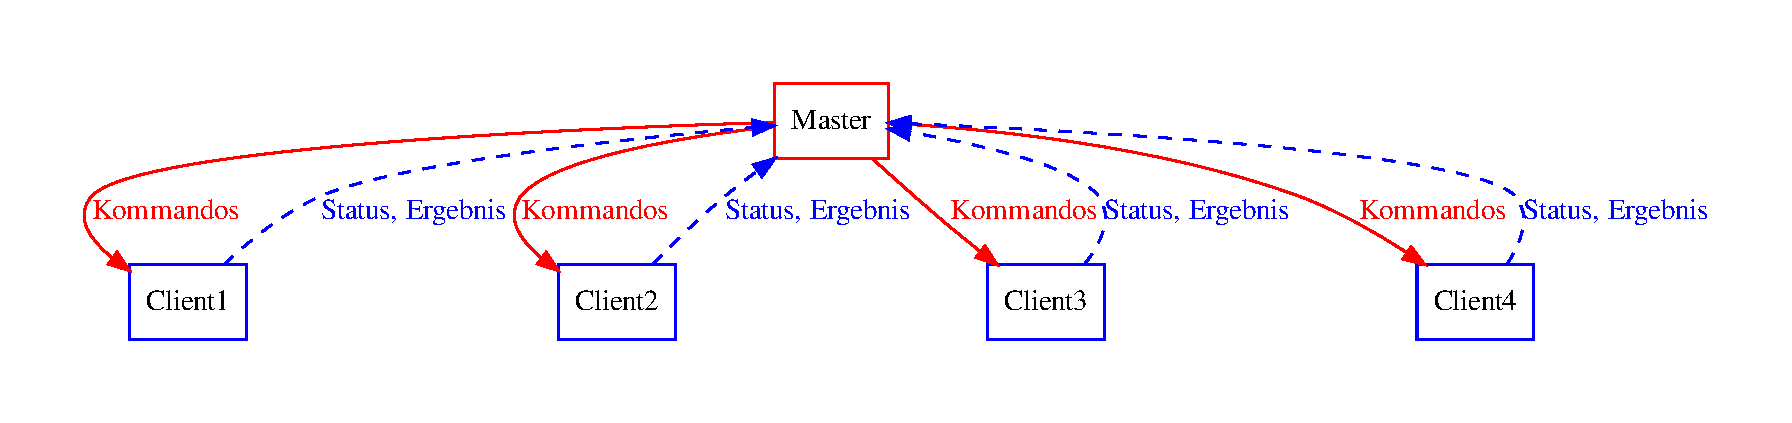
\includegraphics[scale=0.42]{4}}
	\end{figure}
\end{frame}

\subsection{Master}
\begin{frame}
	\ftitle
	\begin{itemize}
		\item Stellt Weboberfläche für die Nutzer*innen zur Verfügung\pause
		\item Überwacht den Status der Clients\pause
		\item Erlaubt Konfiguration der Clients\pause
		\item Programmieren des Ablaufplans\pause
	\end{itemize}
	\vspace{0.5cm}
	\begin{figure}
		\centering
		
\includegraphics[scale=0.1]{django}
		\hspace{3cm}
		
\includegraphics[scale=0.05]{python}
	\end{figure}
\end{frame}

\subsection{Client}
\begin{frame}
	\ftitle
	\begin{itemize}
		\item Erhält Anweisungen vom Server und führt sie aus\pause
		\item Meldet Status zurück an Server\pause
		\item Ansteuerung über RPC-Schnittstelle\pause
	\end{itemize}
	\vspace{0.5cm}
	\begin{figure}
		\centering
		
\includegraphics[scale=0.05]{python}
	\end{figure}
\end{frame}

\section{Entwicklung}
\subsection{Lizenz}

\begin{frame}
	\ftitle
	\adjustbox{valign=t}{
		\begin{minipage}{0.4\textwidth}
			\centering
			
\includegraphics[width=0.9\textwidth]{mit}
		\end{minipage}}
	\begin{minipage}[t]{0.5\textwidth}
		\begin{itemize}
			\item MIT-Lizenz\pause
			\item Sehr offene Lizenz\pause
			\item Erlaubt weitere Verwendung, ohne das der Code veröffentlicht werden muss
		\end{itemize}
	\end{minipage}
\end{frame}

\subsection{Git}

\begin{frame}
	\ftitle
	\adjustbox{valign=t}{
		\begin{minipage}{0.4\textwidth}
			\centering
			
\includegraphics[width=0.9\textwidth]{github}
		\end{minipage}}
	\begin{minipage}[t]{0.5\textwidth}
		\begin{itemize}
			\item Versionsverwaltung\pause
			\item Entwicklung öffentlich\pause
			\item Github-Organisation: \\\url{https://github.com/bp-flugsimulator}
		\end{itemize}
	\end{minipage}
\end{frame}

\subsection{Github}
\begin{frame}
	\ftitle
	\begin{itemize}
		\item Mehrere Repos (Client, Server, QS, Ideen, ...)\pause
		\item User Storys werden als Pull-Requests modelliert\pause
		\item Gewünschte Features werden mit Github Issues modelliert\pause
		\item Übersicht über Kanban-ähnliches Board\pause
	\end{itemize}
\end{frame}

\begin{frame}
	\ftitle
	\begin{figure}
		\centering
		\vspace{-.5cm}
		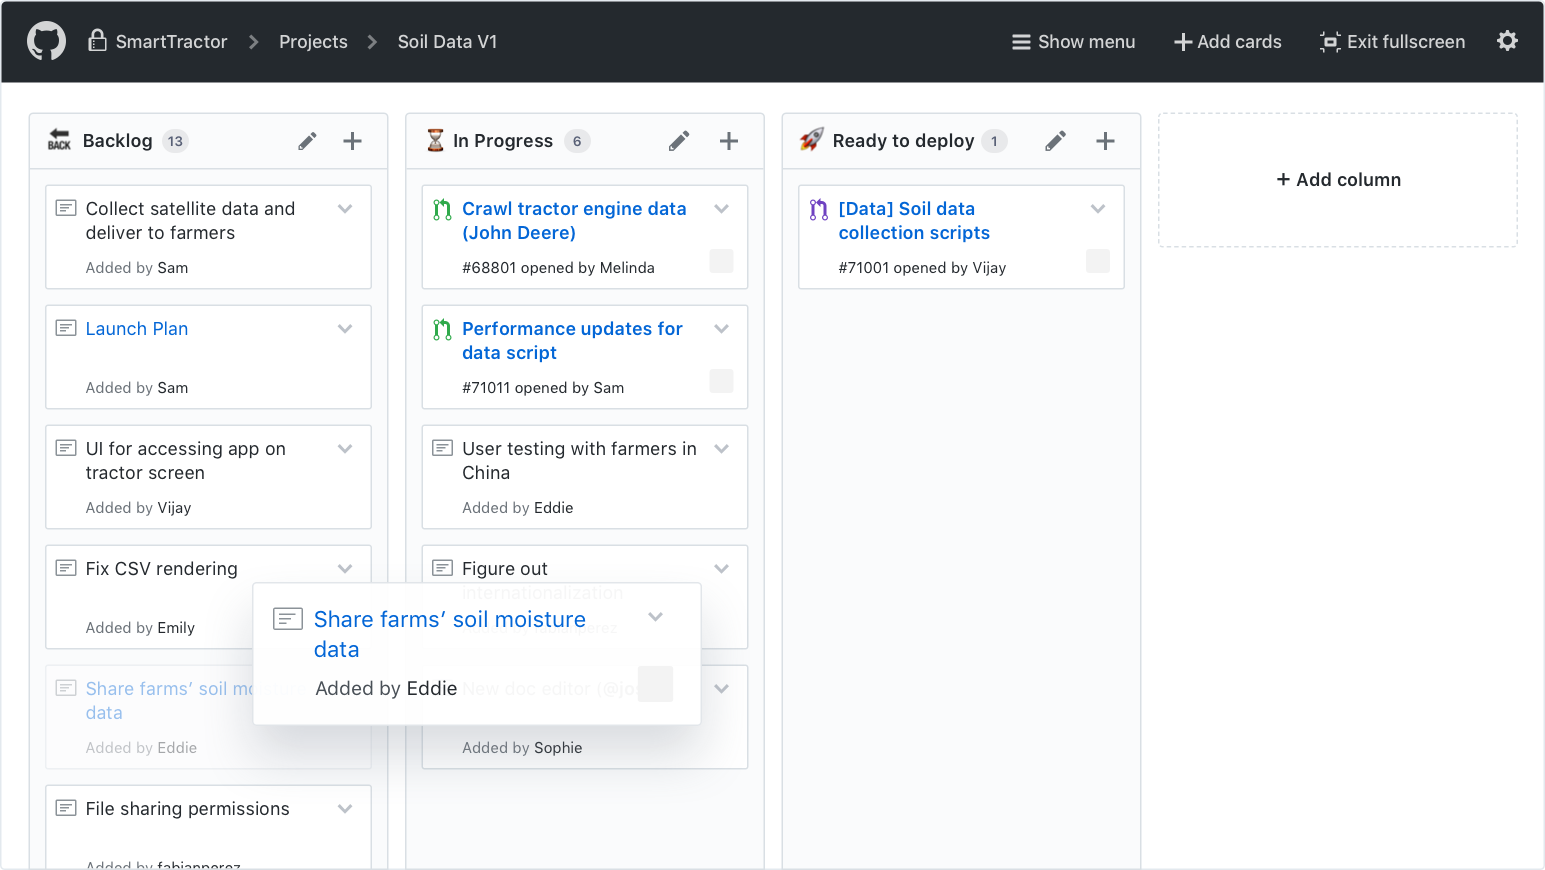
\includegraphics[scale=.2]{projects}
	\end{figure}
\end{frame}

\section{Qualitätssicherung}
\subsection{Testing}

\begin{frame}
	\ftitle
	\begin{itemize}
		\item Nach jedem Commit werden automatisierte Tests durchgeführt\pause
		\item Codestil wird überprüft und eventuell bemängelt\pause
		\item Tests unter Linux und Windows XP\pause
		\item Codestilüberprüfung mit \textbf{yapf}\pause
		\item Testabdeckung mit \textbf{coverage}\pause
	\end{itemize}
			\begin{figure}
				\centering
				
\includegraphics[scale=0.3]{jenkins}
			\end{figure}
\end{frame}

\begin{frame}
	\ftitle
	\begin{figure}
		\centering
		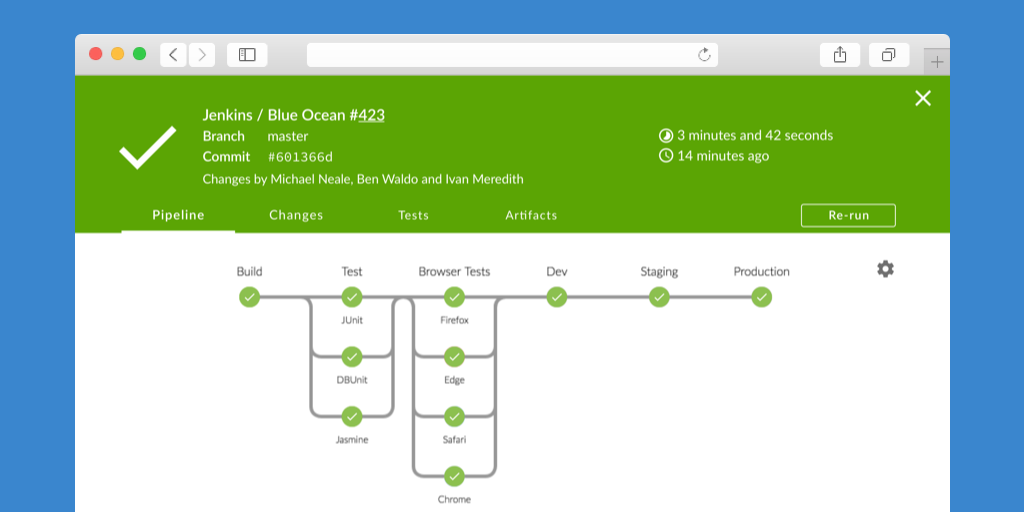
\includegraphics[width=0.9\linewidth]{pipeline}
	\end{figure}
\end{frame}

\subsection{Zeittracking}
\begin{frame}
	\ftitle
	\begin{itemize}
		\item Jedes Teammitglied trackt seine Zeit\pause
		\item Sammeln über Listen im QS-Repo
	\end{itemize}
\end{frame}
\end{document}
